\documentclass{beamer}
\usepackage[latin1]{inputenc}

\usepackage[noend]{algpseudocode}
\usepackage[ruled]{algorithm}
\usepackage{url}
\usepackage{framed}
\usepackage{amsfonts,amsmath,amsthm}
\usepackage{graphicx}
\usepackage{url}
\usepackage{color}

\title{Rational Deployment of CSP Heuristics}
\author{David Tolpin, Solomon Eyal Shimony}
\institute{Ben-Gurion University of the Negev\\Beer Sheva, Israel}
\date{June 1, 2011}

\AtBeginSection[]
{
  \begin{frame}<beamer>
    \frametitle{Outline}
    \tableofcontents[currentsection]
  \end{frame}
}


\begin{document}

\begin{frame}
\titlepage
\end{frame}

\section{Introduction}

\begin{frame}{Introduction}
\begin{itemize}
\item Heuristics are crucial tools in decreasing search effort in
  various areas of AI.
\item A heuristic must provide {\bf useful information} to the search algorithm,
  and be {\bf efficient} to compute.
\item Overhead of some well-known heuristics may outweigh the gain.
\item Such heuristics should be deployed selectively, based on
  principles of {\it rational metareasoning}.
\end{itemize}

\end{frame}

\begin{frame}{Case Study: Constraint Satisfaction}
\begin{itemize}
\item CSP backtracking search algorithms typically employ
  variable-ordering and value-ordering heuristics.
\item Many value ordering heuristics are computationally
  heavy, e.g. heuristics {\it based on solution count
          estimates.}
\item Principles of rational metareasoning can be applied
          to decide when to deploy the heuristics.
\end{itemize}
\end{frame}

\section{Background}

\begin{frame}{Rational Metareasoning}
\begin{itemize}
\item A problem-solving agent can perform {\it base-level} actions from a known
          set $\{A_i\}$.
\item Before committing to an action, the agent may perform a sequence of
          {\it meta-level} deliberation actions from a set $\{S_j\}$.
\item At any given time there is a base-level action $A_\alpha$ that maximizes
          the agent's {\it expected utility.}
\end{itemize}

          The {\bf net VOI $V(S_j)$} of action $S_j$ is the {\bf intrinsic VOI} $\Lambda_j$ less the cost of $S_j$:
          \[V(S_j)=\Lambda(S_j)-C(S_j)\]
           \[\Lambda(S_j)=\mathbb{E}\left(\mathbb{E}(U(A_\alpha^j))-\mathbb{E}(U(A_\alpha))\right)\]

\begin{itemize} 
\item  $S_{j_{\max}}$ that maximizes the net VOI  is performed: $j_{\max} = \arg\max_jV(S_j)$, if $V(S_{j_{\max}})>0$.
\item Otherwise, $A_\alpha$ is performed.
\end{itemize}
\end{frame}

\begin{frame}{Constraint Satisfaction}
A constraint satisfaction problem (CSP) is defined by:
\begin{itemize}
\item[] {\bf variables} $\mathcal{X}=\{X_1, X_2, ...\}$, 
\item[] {\bf constraints} $\mathcal{C}=\{C_1, C_2, ...\}$. 
\end{itemize}
\begin{itemize}
 \item Each {\it variable} $X_i$ has a non-empty domain
          $D_i$ of possible values. 
\item Each {\it constraint} $C_i$ involves some subset
          of the variables---the {\it scope} of the constraint---and specifies the
          allowable combinations of values for that subset. 
\item An {\it assignment} that does not violate any constraints is called
          {\it consistent} (or solution).
 \end{itemize}
 \end{frame}

\section{Rational Value Ordering}

\begin{frame}{Value Ordering Model}
Value ordering heuristics provide information about:
\begin{itemize}
 \item $T_i$---the expected time to find a solution containing
          an assignment  $X_k=y_{ki};$
\item $p_i$---the probability that there is no solution
  consistent with $X_k=y_{ki}$.
\end{itemize}
The expected remaining search time in the subtree under $X_k$ for
ordering $\omega$ is $T^{s|\omega}=T_{\omega(1)}+\sum_{i=2}^{|D_k|}T_{\omega(i)}\prod_{j=1}^{i-1}p_{\omega(j)}$
\begin{itemize}
\item The current optimal base-level action is picking the $\omega $ which optimizes $T^{s|\omega}$.  $T^{s|\omega}$ is minimal if the values are sorted  by increasing order of $\frac {T_i} {1-p_i}$.
\item The intrinsic VOI $\Lambda_i$ of estimating $T_i, p_i$ for the $i$th assignment is the expected decrease in the expected search time:
          $\Lambda_i=\mathbb{E}\left[T^{s|\omega_-}-T^{s|\omega_{+i}}\right]$.
\end{itemize}
\end{frame}

\begin{frame}{Main Results}

{\large{\bf Rational Value Ordering}}

The intrinsic VOI $\Lambda_i$ of invoking the heuristic can be approximated as:
\[\Lambda_i\approx \mathbb{E}\left[(T_1-T_i)|D_k|\,\Big|\; T_i < T_1 \right]\]

{\large{\bf VOI of Solution Count Estimates}}

The net VOI $V$ of estimating a solution count can be approximated as:
\[V \propto |D_k|e^{-\nu}\sum_{n=n_\mathrm{max}}^\infty \! \! \left( \frac 1 {n_\mathrm{max}} - \frac 1 n\right) \frac {\nu^n} {n!}-\gamma\]
where the constant $\gamma$ \textcolor{blue}{depends on the search algorithm and the heuristic, rather than on the CSP instance,} and can be learned offline. 
\end{frame}

\begin{frame}{Alogirthm: SC-based Rational Value Ordering}
\begin{algorithmic}[1]
\Procedure{ValueOrdering-SC}{$csp, X_k, N$}\label{alg:csp-solcount-args}
  \State $D \gets D_k$,\hspace{1em}$n_\mathrm{max} \gets \frac N {|D|}$
  \State {\bf for all} {$i$ {\bf in} $1..|D|$} {\bf do} $n_i \gets n_\mathrm{max}$
  \While {$V(n_\mathrm{max})>0$} \label{alg:csp-solcount-while}
    \State choose $y_{ki} \in D$ arbitrarily
    \State $D \gets D \setminus \{y_{ki}\}$
    \State $csp' \gets csp$ with $D_k=\{y_{ki}\}$
    \State $n_i \gets$ {\sc EstimateSolutionCount}($csp'$) \label{alg:csp-estimate-solution-count}
    \State {\bf if} {$n_i>n_\mathrm{max}$} {\bf then} $n_\mathrm{max} \gets n_i$
  \EndWhile \label{alg:csp-solcount-endwhile}
  \State {\bf end while}
  \State $D_{ord} \gets$ sort $D_k$ by non-increasing $n_i$ \label{alg:csp-solcount-sort}
  \State {\bf return} $D_{ord}$ \label{alg:csp-solcount-return}
\EndProcedure
\end{algorithmic}
\end{frame}

\section{Experiments}

\begin{frame}{Benchmarks}
\vspace{-24pt}
\begin{figure}[h]
\centering
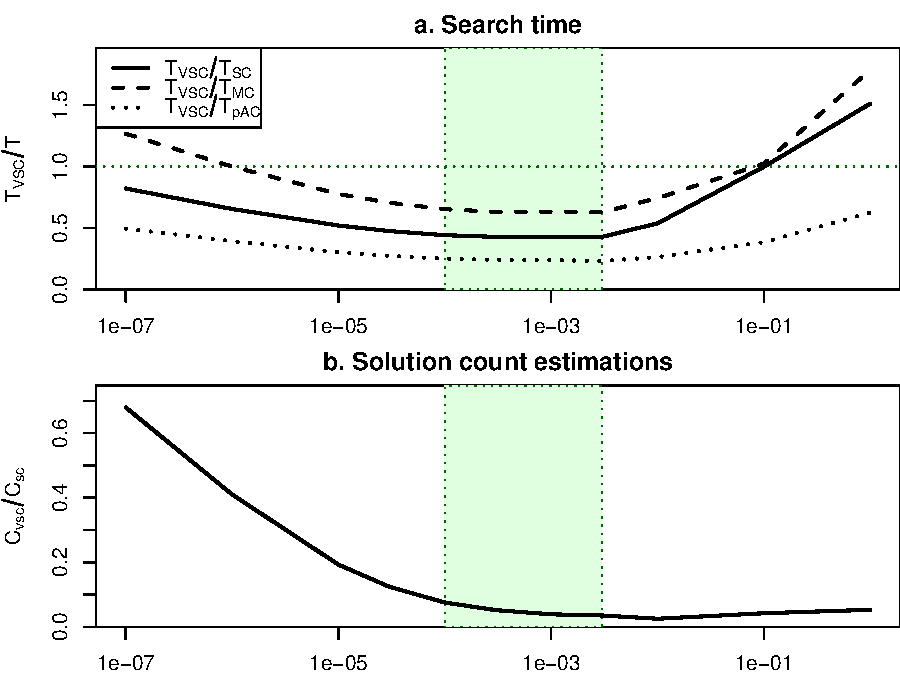
\includegraphics[scale=0.6]{benchmarks.pdf}

14 CSP Solver Competion 2005 Benchmarks\\
solved for $\gamma \in \{0, 10^{-7},$ $10^{-6},$ $...,$ $1\}$
\end{figure}
\end{frame}



\begin{frame}{Random Instances}
\begin{figure}[h] 
\centering
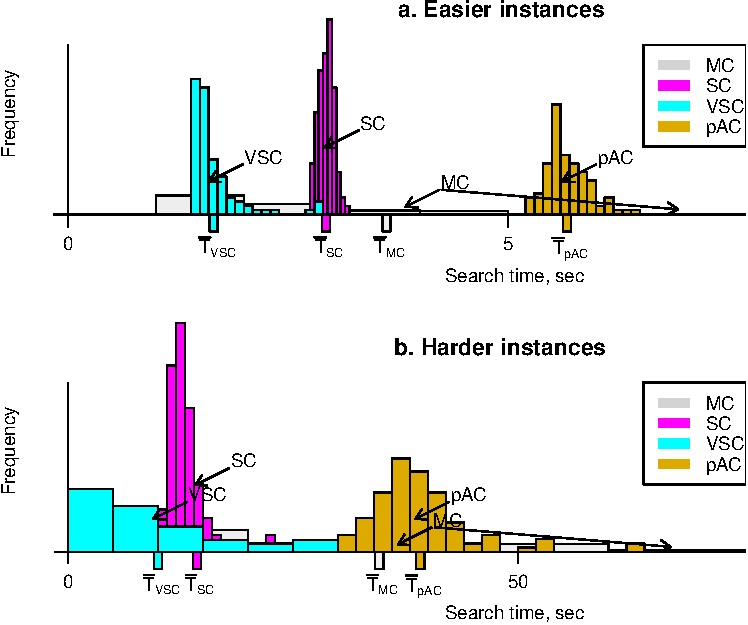
\includegraphics[scale=0.6]{random-problems-arrows+legend.pdf}

100 Model RB Random Instances
\end{figure}
\end{frame}

\begin{frame}{Generalized Sudoku}
\begin{itemize}
\item Real-world problem instances often have much more structure
  than random instances generated according to Model RB.
\item We repeated the
  experiments on randomly generated Generalized Sudoku instances---
  a highly structured domain.
\item Relative performance on Generalized Sudoku was similar to
  Model~RB.
\end{itemize}
\end{frame}

\section{Conclusion}

 \begin{frame}{Summary}
\begin{itemize}
\item This work suggests a {\bf model for adaptive deployment} of value ordering
      heuristics in algorithms for constraint satisfaction problems.
\item As a case study, the model was applied to a value-ordering heuristic based
      on solution count estimates, and a {\it steady improvement}  was achieved
      compared to {\bf always} computing the estimates.  
\item For many problem instances the optimum
      performance is achieved when solution {\bf counts are estimated only in a
      small number of search states.}
\end{itemize}
\end{frame}

\begin{frame}{Future Work}
\begin{itemize}
\item Generalization of the VOI to deploy different types of
  heuristics for CSP.
\item Explicit evaluation of the quality of the distribution model, coupled
  with a better candidate model of the distribution.
\item Application to search in other domains, especially
  to heuristics for planning;  in particular, examining whether
  the meta-reasoning scheme can improve reasoning over deployment based
  solely on learning.
\end{itemize}
\end{frame}

\end{document}
